\documentclass[aspectratio=169,unicode,dvipdfmx,14pt]{beamer}


\usepackage{url}
\usepackage{bm}
\usepackage{amsmath}
\usepackage{amssymb}
\usepackage{mathtools}
\usepackage{graphicx}
\usepackage[absolute,overlay]{textpos}
\usepackage{hyperref}
\usepackage{listings}
\usepackage{changepage}
\usepackage{lipsum}


\usefonttheme[onlymath]{serif}

\DeclareMathOperator*{\argmax}{argmax}

\DeclarePairedDelimiterX{\infdivx}[2]{(}{)}{%
  #1\;\delimsize\|\;#2%
}
\newcommand{\infdiv}{D_{\scriptsize \mbox{KL}}\infdivx}
\DeclarePairedDelimiter{\norm}{\lVert}{\rVert}

\hypersetup{
	setpagesize=false,
	bookmarksnumbered=true,%
	bookmarksopen=true,%
	colorlinks=true,%
	linkcolor=blue,
	citecolor=red,
}

\newcommand\FontMath{\fontsize{10}{12}\selectfont}
\renewcommand{\baselinestretch}{1.3}
\renewcommand{\familydefault}{\sfdefault}
\renewcommand{\kanjifamilydefault}{\gtdefault}
\usepackage[deluxe, expert]{otf}

\setbeamertemplate{navigation symbols}{}
\setbeamertemplate{footline}[frame number]
\setbeamerfont{footline}{size={\fontsize{15}{15}}}

\setbeamerfont{author}{size=\Large}
\setbeamerfont{institute}{size=\normalsize\itshape}
\setbeamerfont{title}{size=\huge}
\setbeamerfont{subtitle}{size=\LARGE\normalfont\slshape}


\title{PLSI \\ (probabilistic latent semantic indexing)}
\author{\texorpdfstring{正田 備也\newline\href{mailto:masada@rikkyo.ac.jp}{masada@rikkyo.ac.jp}}{正田 備也}}
\date{}

\begin{document}

\begin{frame}
\titlepage
\end{frame}

\section{混合多項分布の問題点}

\begin{frame}\frametitle{Contents}
\Large \tableofcontents[currentsection]
\end{frame}

\begin{frame}{混合多項分布}
\begin{itemize}
\item 混合多項分布モデルでは、一つ一つの文書がそれ全体で、意味的なまとまりを持つ
\begin{itemize}
\item ニュース記事であれば、記事まるごと、特定のカテゴリ(ex. 政治、経済、スポーツ、etc)に割り振られる。
\end{itemize}
\item つまり、一つの文書内は意味的に均一だと、仮定している
\item しかし、この仮定は現実の文書の実態に合わない
\begin{itemize}
\item 文書は複数の話題を含みうるので。
\end{itemize}
\end{itemize}
\end{frame}

\begin{frame}{混合多項分布の改良}
\begin{itemize}
\item カテゴリの違いは、混合多項分布と同様、語彙集合上に定義された多項分布(単語多項分布)の違いとして表す
\begin{itemize}
\item 政治について書かれたテキストと、スポーツについて書いたテキストとでは、どの単語がどのくらいの確率で出現するかが異なる、という考え方。
\end{itemize}
\item そこで、一つの文書に含まれる単語トークン群が、唯一の単語多項分布からではなく、複数の単語多項分布から生成されると、仮定する→\underline{PLSIモデル}
\begin{itemize}
\item 同じ文書内に、異なる単語多項分布に由来する単語トークンが混ざっていてもよい、という考え方。
\end{itemize}
\end{itemize}
\end{frame}

\begin{frame}
\begin{figure}[htbp]
\begin{center}
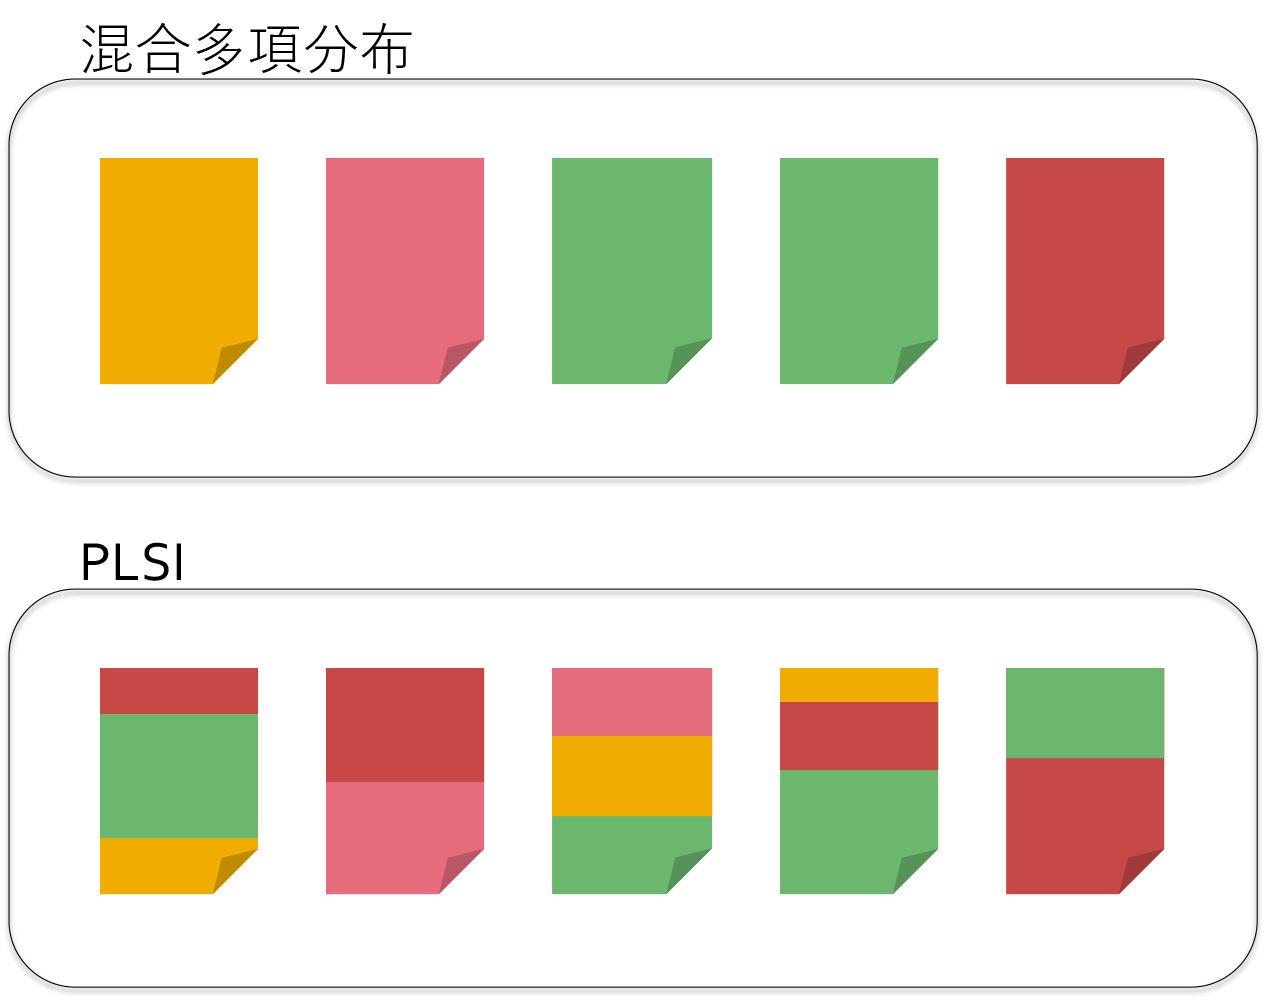
\includegraphics[scale=.21]{PLSI1.jpg}
\caption{混合多項分布とPLSIの違い}
\label{}
\end{center}
\end{figure}\end{frame}

\begin{frame}
\begin{figure}[htbp]
\begin{center}
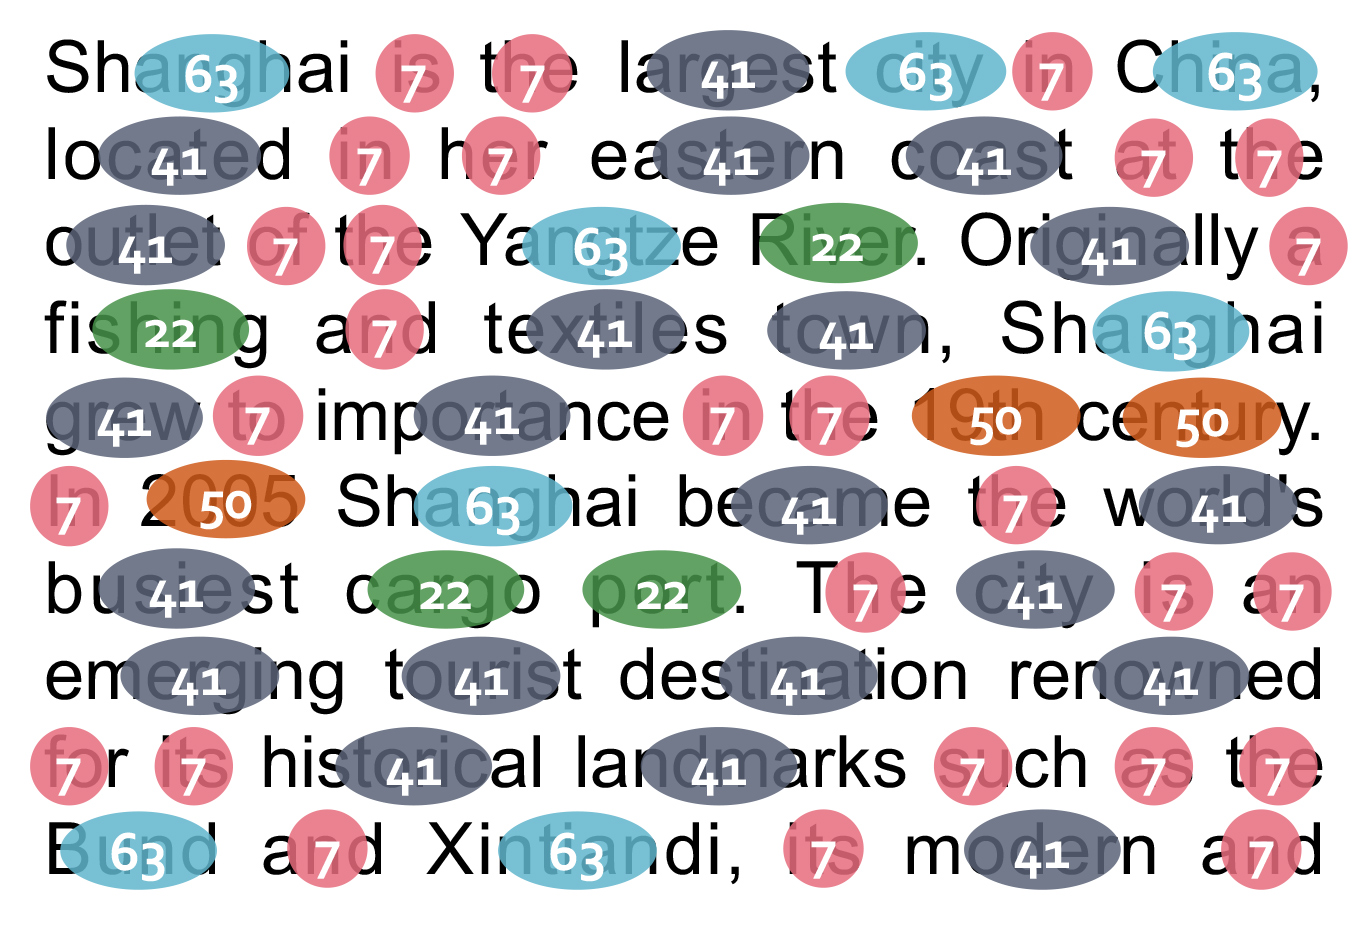
\includegraphics[scale=.22]{PLSI2.jpg}
\vspace{-.2in}
\caption{PLSIでは同じ文書の単語トークンが複数の単語多項分布に由来}
\label{}
\end{center}
\end{figure}
\end{frame}

\section{PLSI}

\begin{frame}\frametitle{Contents}
\Large \tableofcontents[currentsection]
\end{frame}

\begin{frame}{PLSI (probabilistic latent semantic indexing)}
\begin{itemize}
\item LSI(latent semantic indexing)確率モデル化したモデル
\begin{itemize}
\item LSIについては、説明を割愛(実態は単なるSVD)
\end{itemize}
\item 同じ文書内でも、単語トークンが異なる単語多項分布から生成される
\item どの単語多項分布がどのくらいの確率で使われるかが、文書によって異なる
\item PLSIにおける単語多項分布を、トピック(topic)と呼ぶ
\begin{itemize}
\item PLSIは最もシンプルなトピックモデル
\end{itemize}
\end{itemize}
\end{frame}

\begin{frame}{確率モデル}
\end{frame}


\end{document}